\documentclass[11pt, english]{article}

\usepackage{multicol}
\usepackage{hyperref}
\usepackage[eng]{felipito}
\usepackage{stfloats}
\usepackage{mathpazo}

\usepackage[margin=0.7in, left=0.7in, right=0.7in]{geometry}

\graphicspath{{./Graphics/}}

% Colors
\definecolor{urlcolor}{rgb}{0,.145,.698}
\definecolor{linkcolor}{rgb}{.71,0.21,0.01}
\definecolor{citecolor}{rgb}{.12,.54,.11}


% Document title
\title{\bf Problem Set 5 \\ Statistics, Computation and
Applications\\[-1ex]}
\author{Felipe del Canto}
\date{November, 2021}
    
\hypersetup{
	breaklinks=true,  % so long urls are correctly broken across lines
    colorlinks=true,
    urlcolor=urlcolor,
    linkcolor=linkcolor,
    citecolor=citecolor,
}

\begin{document}
    
\maketitle
   
\begin{multicols}{2}

\section*{Problem 5.1: Flows and Correlations}

For parts (a) and (b), the first step is to compute the average flow over time. The grid used implies that each coordinate covers a 3km grid. Additionally, all flow values are expressed in cm/second (cmps). In order to gain a better sense of the strength of the currents, two different average speeds are computed. First, the speed of the average flow. This is, compute the speed \textit{after} averaging the flow vectors. Second, the average of all speed values over time. In other words, the speed is \textit{before} averaging. In \Cref{fig:flow-speed} it is presented the first of these two speed representations. The fastest flow runs from east to west on the southern end of the Archipielago (around 900 km east of the initial coordinate). There is also a strong current around the islands to the southwest (around 300 km north of the initial coordinate) Other important flows run on the east, mostly going south. There are lesser important but prevalent currents running almost in circular patterns at the center and the west and at the center-north, on the east. In contrast, in \Cref{fig:flow-speed-2} is presented the second of the speed representations. In this case, the speed of the flow at each time is computed and then averaged over time. The patters shown in the previous picture still hold. The most strong currents are present in the southern part of the Archipielago, and in the islands at the south west (around 900 km to the north of the initial coordinates).

\begin{figure*}
	\caption{Average flow and speed flow for a zone of the Philippines Archipielago. In panel (a), the rows represent the average flow over time. The colors on the arrows represent the speed of the flow (i.e., the size of the arrow) in cmps. In panel (b), the colors represent the average speed over time, that is, averaging the speed of the flow at each time.}
	\label{fig:flow}
	\begin{subfigure}{0.48\textwidth}
		\centering
		\caption{Average flow and speed}
		\label{fig:flow-speed}
		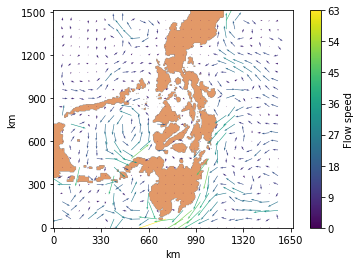
\includegraphics[width=\textwidth]{flow-speed}
	\end{subfigure}\hfill
	\begin{subfigure}{0.48\textwidth}
		\centering
		\caption{Average speed over time}
		\label{fig:flow-speed-2}
		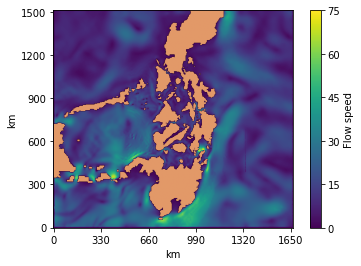
\includegraphics[width=\textwidth]{flow-speed-2}
	\end{subfigure}
\end{figure*}


For part (c), the main goal is to understand if a Gaussian Process (GP) might be a good model for making predictions about currents in the Archipielago. For this, spatial correlations must be understood. To this end, two coordinates are considered and the flow and speed correlations with their surroundings are studied. The two coordinates are (420 km, 345 km) and (1200 km, 1200 km). Moreover, the correlations are computed for three variables: the horizontal flow, the vertical flow and the speed. In \Cref{fig:coord} are presented the results for both coordinates. In particular, panels (a) to (c) show the correlations for the first coordinate. These figures show that horizontal flow is more diverse in terms of correlation, with zones close to the point of reference that have high and low correlation values. On the opposite side, the vertical component of the flow is in general more positively correlated with the reference point. In particular, the previous observation suggests that a GP would not be a reasonable model for the horizontal component of the flow. This, because the red zones are roughly at the same distance that other blue zones. If a GP with covariances following a kernel modelled these zones, then both should have the same color. Additionally, the zones south of the reference point do not seem correlated with it, mounting more evidence against a GP model. In contrast, the vertical component and speed images do have a more stable behavior in terms of the neighbors of the reference point. However, the same concern regarding zones more to the south suggests that GP is not a good model. Now, we turn to the surroundings of the second coordinate, which are shown in \Cref{fig:coord-2-h,fig:coord-2-v,fig:coord-2-s}. These panels show a completely different story. Around the reference point, the correlations are spurious. In particular, the zones closer to the point have almost zero correlation. In that sense, it could be argued that in this case, GP are a good model. However, the small correlations would imply a very poor predictive power, making the model useless nonetheless. In the other hand, the caveat is that even if the surroundings of the reference point do follow a distance-driven covariance pattern, points further away have nonzero correlations. If a GP were to model this data, the correlation between the reference point and these far away points should be smaller than those closer, which is not the case. All in all, the analysis of the previous two coordinates suggests that a GP would not be a good model for this data. The reason might be that currents form a complex system, with difficult rules. If these rules are nonlinear, then correlations, that are more suited for linear dependencies, fail to capture the underlying phenomena.



\begin{figure*}
	\caption{Spatial correlations for coordinates (420 km, 345 km) and (1200 km, 1200 km). Panels (a)-(c) show the correlations of the first coordinate and its surroundings for horizontal flow, vertical flow, and speed, respectively. Analogously, panels (d)-(f) show the same for the second coordinate. In all panels, the green dot represents the corresponding coordinate.}
	\label{fig:coord}
	\begin{subfigure}{0.33\textwidth}
		\centering
		\caption{Horizontal flow.}
		\label{fig:coord-1-h}
		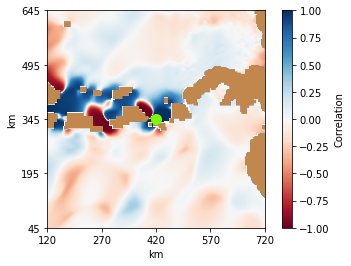
\includegraphics[width=\textwidth]{coord-1-h}
	\end{subfigure}\hfill
	\begin{subfigure}{0.33\textwidth}
		\centering
		\caption{Vertical flow.}
		\label{fig:coord-1-v}
		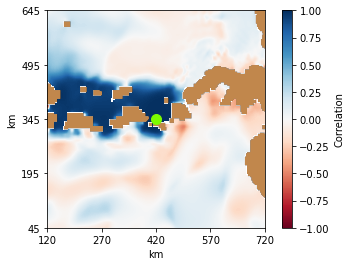
\includegraphics[width=\textwidth]{coord-1-v}
	\end{subfigure}
	\begin{subfigure}{0.33\textwidth}
		\centering
		\caption{Speed.}
		\label{fig:coord-1-s}
		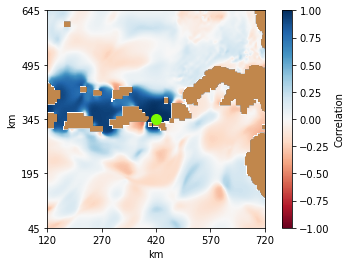
\includegraphics[width=\textwidth]{coord-1-s}
	\end{subfigure}\vspace{2ex}
	
	\begin{subfigure}{0.33\textwidth}
		\centering
		\caption{Horizontal flow.}
		\label{fig:coord-2-h}
		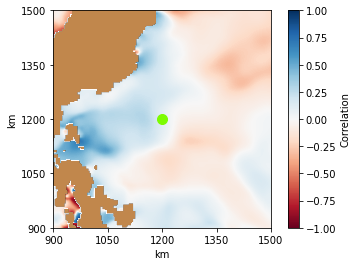
\includegraphics[width=\textwidth]{coord-2-h}
	\end{subfigure}\hfill
	\begin{subfigure}{0.33\textwidth}
		\centering
		\caption{Vertical flow.}
		\label{fig:coord-2-v}
		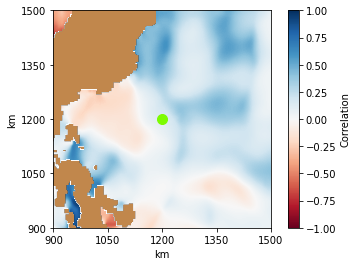
\includegraphics[width=\textwidth]{coord-2-v}
	\end{subfigure}
	\begin{subfigure}{0.33\textwidth}
		\centering
		\caption{Speed.}
		\label{fig:coord-2-s}
		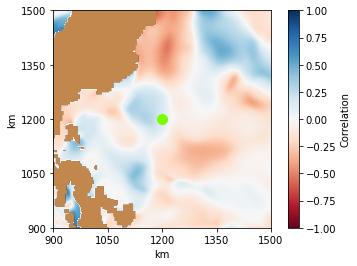
\includegraphics[width=\textwidth]{coord-2-s}
	\end{subfigure}
\end{figure*}

\section*{Problem 5.2: Predicting Trajectories}

For part (a),

For part (b),


\section*{Problem 5.3: Gaussian Processes}

For part (a), consider the squared exponential/RBF covariance function
	$$\kappa(x_{i}, x_{j}) = \sigma^{2}\exp\left(-\frac{(x_{i} - x_{j})^{2}}{2\ell^{2}}\right),$$
where $\sigma^2$ is the signal variance and $\ell$ is the lengthscale. If the signal variance is increased, then all things equal, points will have a higher covariance. In other words, the covariance curve (as a function of distance $|x_{i} - x_{j}|$) is higher, the higher $\sigma^{2}$ is. This is shown in \Cref{fig:rbf-sigma}. Moreover, the image shows the decay is similar among all three functions, reaching values close to zero when the distance is close to 3. On the other hand, varying the lengthscale has different effects on the covariance function. As shown in \Cref{fig:rbf-ell}, changing the lengthscale drastically affects the decaying rate of the function. When $\ell$ is small, the decay is faster than when it is larger.

\begin{figure*}
	\caption{Effect of $\sigma^{2}$ and $\ell$ on the RBF covariance function $\kappa(x_{i}, x_{j})$. Panel (a) shows the effect of varying $\sigma^{2}$, when holding $\ell = 1$ constant. In panel (b) it is shown the effect of varying $\ell$, holding $\sigma^{2} = 1$ constant.}
	\label{fig:rbf}
	\begin{subfigure}{0.48\textwidth}
		\centering
		\caption{$\ell = 1$}
		\label{fig:rbf-sigma}
		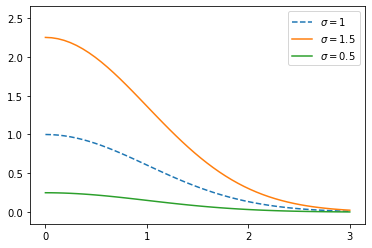
\includegraphics[width=\textwidth]{rbf-sigma}
	\end{subfigure}\hfill
	\begin{subfigure}{0.48\textwidth}
		\centering
		\caption{$\sigma^{2} = 1$}
		\label{fig:rbf-ell}
		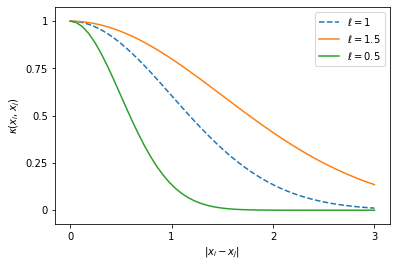
\includegraphics[width=\textwidth]{rbf-ell}
	\end{subfigure}
\end{figure*}


For part (b), suppose we have data points $\{(x_{i}, y_{i})\}_{i=1}^{N}$, where $x_{i}$ are locations and $y_{i}$ are given outcomes. Additionally, we have a new observation $x_{*}$ for which we wish to estimate $y_{*}$. A Gaussian Process (GP) model assumes each $y_{i}$ is drawn from $Y_{i}$ and that $Y := (Y_{1}, \ldots, Y_{N}, Y_{*})$ follows a multivariate normal distribution. Let $\mu$ and $\Sigma$ be the mean and covariance matrix of that distribution and assume $\mu = 0$. Let $\sigma_{*}$ be the variance of $Y_{*}$, $\sigma_{N}$ be the $N \times N$ top left block of $\Sigma$, and let $k^{*}$ be the vector whose entries are $k(x_{*}, x_{i})$, where $k$ is the kernel function that is used to model the covariances. Then, the parameters for the distribution of $Y_{*}$ are:
	\begin{align*}
		\mu_{*\,|\,1:N}		&=	k_{*}^{T}K_{N}^{-1}y_{1:N}	\\
		\sigma_{*}\,|\,1:N	&=	\sigma_{*} - k_{*}^{T}K_{N}^{-1}k_{*}
	\end{align*}
Observe that computing both parameters implies that the matrix $K_{N}$ has to be inverted. If $N$ is large, this operation can take large amounts of time or even be impossible to do due to memory restrictions.


For part (c), 




\end{multicols}
\end{document}
